%  LaTeX support: latex@mdpi.com 
%  For support, please attach all files needed for compiling as well as the log file, and specify your operating system, LaTeX version, and LaTeX editor.

%=================================================================
\documentclass[journal,article,submit,pdftex,moreauthors]{Definitions/mdpi} 

%--------------------
% Class Options:
%--------------------
%----------
% journal
%----------
% Choose between the following MDPI journals:
% acoustics, actuators, addictions, admsci, adolescents, aerobiology, aerospace, agriculture, agriengineering, agrochemicals, agronomy, ai, air, algorithms, allergies, alloys, analytica, analytics, anatomia, animals, antibiotics, antibodies, antioxidants, applbiosci, appliedchem, appliedmath, applmech, applmicrobiol, applnano, applsci, aquacj, architecture, arm, arthropoda, arts, asc, asi, astronomy, atmosphere, atoms, audiolres, automation, axioms, bacteria, batteries, bdcc, behavsci, beverages, biochem, bioengineering, biologics, biology, biomass, biomechanics, biomed, biomedicines, biomedinformatics, biomimetics, biomolecules, biophysica, biosensors, biotech, birds, bloods, blsf, brainsci, breath, buildings, businesses, cancers, carbon, cardiogenetics, catalysts, cells, ceramics, challenges, chemengineering, chemistry, chemosensors, chemproc, children, chips, cimb, civileng, cleantechnol, climate, clinpract, clockssleep, cmd, coasts, coatings, colloids, colorants, commodities, compounds, computation, computers, condensedmatter, conservation, constrmater, cosmetics, covid, crops, cryptography, crystals, csmf, ctn, curroncol, cyber, dairy, data, ddc, dentistry, dermato, dermatopathology, designs, devices, diabetology, diagnostics, dietetics, digital, disabilities, diseases, diversity, dna, drones, dynamics, earth, ebj, ecologies, econometrics, economies, education, ejihpe, electricity, electrochem, electronicmat, electronics, encyclopedia, endocrines, energies, eng, engproc, entomology, entropy, environments, environsciproc, epidemiologia, epigenomes, est, fermentation, fibers, fintech, fire, fishes, fluids, foods, forecasting, forensicsci, forests, foundations, fractalfract, fuels, future, futureinternet, futurepharmacol, futurephys, futuretransp, galaxies, games, gases, gastroent, gastrointestdisord, gels, genealogy, genes, geographies, geohazards, geomatics, geosciences, geotechnics, geriatrics, grasses, gucdd, hazardousmatters, healthcare, hearts, hemato, hematolrep, heritage, higheredu, highthroughput, histories, horticulturae, hospitals, humanities, humans, hydrobiology, hydrogen, hydrology, hygiene, idr, ijerph, ijfs, ijgi, ijms, ijns, ijpb, ijtm, ijtpp, ime, immuno, informatics, information, infrastructures, inorganics, insects, instruments, inventions, iot, j, jal, jcdd, jcm, jcp, jcs, jcto, jdb, jeta, jfb, jfmk, jimaging, jintelligence, jlpea, jmmp, jmp, jmse, jne, jnt, jof, joitmc, jor, journalmedia, jox, jpm, jrfm, jsan, jtaer, jvd, jzbg, kidneydial, kinasesphosphatases, knowledge, land, languages, laws, life, liquids, literature, livers, logics, logistics, lubricants, lymphatics, machines, macromol, magnetism, magnetochemistry, make, marinedrugs, materials, materproc, mathematics, mca, measurements, medicina, medicines, medsci, membranes, merits, metabolites, metals, meteorology, methane, metrology, micro, microarrays, microbiolres, micromachines, microorganisms, microplastics, minerals, mining, modelling, molbank, molecules, mps, msf, mti, muscles, nanoenergyadv, nanomanufacturing,\gdef\@continuouspages{yes}} nanomaterials, ncrna, ndt, network, neuroglia, neurolint, neurosci, nitrogen, notspecified, %%nri, nursrep, nutraceuticals, nutrients, obesities, oceans, ohbm, onco, %oncopathology, optics, oral, organics, organoids, osteology, oxygen, parasites, parasitologia, particles, pathogens, pathophysiology, pediatrrep, pharmaceuticals, pharmaceutics, pharmacoepidemiology,\gdef\@ISSN{2813-0618}\gdef\@continuous pharmacy, philosophies, photochem, photonics, phycology, physchem, physics, physiologia, plants, plasma, platforms, pollutants, polymers, polysaccharides, poultry, powders, preprints, proceedings, processes, prosthesis, proteomes, psf, psych, psychiatryint, psychoactives, publications, quantumrep, quaternary, qubs, radiation, reactions, receptors, recycling, regeneration, religions, remotesensing, reports, reprodmed, resources, rheumato, risks, robotics, ruminants, safety, sci, scipharm, sclerosis, seeds, sensors, separations, sexes, signals, sinusitis, skins, smartcities, sna, societies, socsci, software, soilsystems, solar, solids, spectroscj, sports, standards, stats, std, stresses, surfaces, surgeries, suschem, sustainability, symmetry, synbio, systems, targets, taxonomy, technologies, telecom, test, textiles, thalassrep, thermo, tomography, tourismhosp, toxics, toxins, transplantology, transportation, traumacare, traumas, tropicalmed, universe, urbansci, uro, vaccines, vehicles, venereology, vetsci, vibration, virtualworlds, viruses, vision, waste, water, wem, wevj, wind, women, world, youth, zoonoticdis 
% For posting an early version of this manuscript as a preprint, you may use "preprints" as the journal. Changing "submit" to "accept" before posting will remove line numbers.

%---------
% article
%---------
% The default type of manuscript is "article", but can be replaced by: 
% abstract, addendum, article, book, bookreview, briefreport, casereport, comment, commentary, communication, conferenceproceedings, correction, conferencereport, entry, expressionofconcern, extendedabstract, datadescriptor, editorial, essay, erratum, hypothesis, interestingimage, obituary, opinion, projectreport, reply, retraction, review, perspective, protocol, shortnote, studyprotocol, systematicreview, supfile, technicalnote, viewpoint, guidelines, registeredreport, tutorial
% supfile = supplementary materials

%----------
% submit
%----------
% The class option "submit" will be changed to "accept" by the Editorial Office when the paper is accepted. This will only make changes to the frontpage (e.g., the logo of the journal will get visible), the headings, and the copyright information. Also, line numbering will be removed. Journal info and pagination for accepted papers will also be assigned by the Editorial Office.

%------------------
% moreauthors
%------------------
% If there is only one author the class option oneauthor should be used. Otherwise use the class option moreauthors.

%---------
% pdftex
%---------
% The option pdftex is for use with pdfLaTeX. Remove "pdftex" for (1) compiling with LaTeX & dvi2pdf (if eps figures are used) or for (2) compiling with XeLaTeX.

%=================================================================
% MDPI internal commands - do not modify
\firstpage{1} 
\makeatletter 
\setcounter{page}{\@firstpage} 
\makeatother
\pubvolume{1}
\issuenum{1}
\articlenumber{0}
\pubyear{2023}
\copyrightyear{2023}
%\externaleditor{Academic Editor: Firstname Lastname}
\datereceived{ } 
\daterevised{ } % Comment out if no revised date
\dateaccepted{ } 
\datepublished{ } 
%\datecorrected{} % For corrected papers: "Corrected: XXX" date in the original paper.
%\dateretracted{} % For corrected papers: "Retracted: XXX" date in the original paper.
\hreflink{https://doi.org/} % If needed use \linebreak
%\doinum{}
%\pdfoutput=1 % Uncommented for upload to arXiv.org

%=================================================================
% Add packages and commands here. The following packages are loaded in our class file: fontenc, inputenc, calc, indentfirst, fancyhdr, graphicx, epstopdf, lastpage, ifthen, float, amsmath, amssymb, lineno, setspace, enumitem, mathpazo, booktabs, titlesec, etoolbox, tabto, xcolor, colortbl, soul, multirow, microtype, tikz, totcount, changepage, attrib, upgreek, array, tabularx, pbox, ragged2e, tocloft, marginnote, marginfix, enotez, amsthm, natbib, hyperref, cleveref, scrextend, url, geometry, newfloat, caption, draftwatermark, seqsplit
% cleveref: load \crefname definitions after \begin{document}

%=================================================================
% Please use the following mathematics environments: Theorem, Lemma, Corollary, Proposition, Characterization, Property, Problem, Example, ExamplesandDefinitions, Hypothesis, Remark, Definition, Notation, Assumption
%% For proofs, please use the proof environment (the amsthm package is loaded by the MDPI class).

%=================================================================
% Full title of the paper (Capitalized)
\Title{An Approach Using Multiple MLP Neural Networks for Predicting the Brazilian Stock Market}

% MDPI internal command: Title for citation in the left column
\TitleCitation{An Approach Using Multiple MLP Neural Networks for Predicting the Brazilian Stock Market}

% Author Orchid ID: enter ID or remove command
\newcommand{\orcidauthorA}{0000-0000-0000-000X} % Add \orcidA{} behind the author's name
%\newcommand{\orcidauthorB}{0000-0000-0000-000X} % Add \orcidB{} behind the author's name

% Authors, for the paper (add full first names)
% \Author{Paulo Tasinaffo $^{1,\dagger,\ddagger}$\orcidA{} and Luiz Dias $^{2,\ddagger}$}
% ORCID of Tasinaffo, P. M.: https://orcid.org/0000-0001-7069-8430
% ORCID of Dias, L. A. V.: https://orcid.org/0000-0002-6544-7458
\Author{Paulo Tasinaffo$^{1}$ and Luiz Dias}

%\longauthorlist{yes}

% MDPI internal command: Authors, for metadata in PDF
\AuthorNames{Paulo Tasinaffo and Luiz Dias}

% MDPI internal command: Authors, for citation in the left column
\AuthorCitation{Tasinaffo, P. M. ; Dias, L. A. V.}
% If this is a Chicago style journal: Lastname, Firstname, Firstname Lastname, and Firstname Lastname.

% Affiliations / Addresses (Add [1] after \address if there is only one affiliation.)
\address{%
$^{1}$ \quad Instituto Tecnológico de Aeronáutica (ITA), São José dos Campos/SP, Brazil; tasinaffo@ita.br}  % \\
% $^{2}$ \quad Affiliation 2; e-mail@e-mail.com}

% Contact information of the corresponding author
% \corres{Correspondence: e-mail@e-mail.com; Tel.: (optional; include country code; if there are multiple corresponding authors, add author initials) +xx-xxxx-xxx-xxxx (F.L.)}

% Current address and/or shared authorship
% \firstnote{Current address: Affiliation 3.} 
% \secondnote{These authors contributed equally to this work.}
% The commands \thirdnote{} till \eighthnote{} are available for further notes

%\simplesumm{} % Simple summary

%\conference{} % An extended version of a conference paper

% Abstract (Do not insert blank lines, i.e. \\) 
\abstract{The Brazilian stock market undergoes many fluctuations over time. This makes it highly unpredictable. To make matters worse, the 2020 pandemic and financial speculation made the Brazilian stock market even more unpredictable. Therefore, in this article, an approach based on Artificial Intelligence (AI) is proposed to carry out this prediction. For this purpose, multiple MLP neural networks will be coupled, using supervised learning with input/output training patterns through the NARMAX (Nonlinear Auto Regressive Moving Average with eXogenous input) method. A case study, using the actions of the three main companies in Brazil (PETROBRAS, EMBRAER and Vale do Rio Doce) are considered for the validation of the presented methodology. A numerical and computational comparison between the proposed multiple method and the method using only one neural network is also presented.}

% Keywords
\keyword{Universal Numerical Integrator (UNI); Nonlinear Auto Regressive Moving Average with eXogenous input (NARMAX); neural differential equations; Euler-Type Universal Numerical Integrator (E-TUNI); Runge-Kutta Neural Network (RKNN); Adams-Bashforth Neural Network (ABNN)} 

% The fields PACS, MSC, and JEL may be left empty or commented out if not applicable
%\PACS{J0101}
%\MSC{}
%\JEL{}

%%%%%%%%%%%%%%%%%%%%%%%%%%%%%%%%%%%%%%%%%%
% Only for the journal Diversity
%\LSID{\url{http://}}

%%%%%%%%%%%%%%%%%%%%%%%%%%%%%%%%%%%%%%%%%%
% Only for the journal Applied Sciences
%\featuredapplication{Authors are encouraged to provide a concise description of the specific application or a potential application of the work. This section is not mandatory.}
%%%%%%%%%%%%%%%%%%%%%%%%%%%%%%%%%%%%%%%%%%

%%%%%%%%%%%%%%%%%%%%%%%%%%%%%%%%%%%%%%%%%%
% Only for the journal Data
%\dataset{DOI number or link to the deposited data set if the data set is published separately. If the data set shall be published as a supplement to this paper, this field will be filled by the journal editors. In this case, please submit the data set as a supplement.}
%\datasetlicense{License under which the data set is made available (CC0, CC-BY, CC-BY-SA, CC-BY-NC, etc.)}

%%%%%%%%%%%%%%%%%%%%%%%%%%%%%%%%%%%%%%%%%%
% Only for the journal Toxins
%\keycontribution{The breakthroughs or highlights of the manuscript. Authors can write one or two sentences to describe the most important part of the paper.}

%%%%%%%%%%%%%%%%%%%%%%%%%%%%%%%%%%%%%%%%%%
% Only for the journal Encyclopedia
%\encyclopediadef{For entry manuscripts only: please provide a brief overview of the entry title instead of an abstract.}

%%%%%%%%%%%%%%%%%%%%%%%%%%%%%%%%%%%%%%%%%%
% Only for the journal Advances in Respiratory Medicine
%\addhighlights{yes}
%\renewcommand{\addhighlights}{%

%\noindent This is an obligatory section in “Advances in Respiratory Medicine”, whose goal is to increase the discoverability and readability of the article via search engines and other scholars. Highlights should not be a copy of the abstract, but a simple text allowing the reader to quickly and simplified find out what the article is about and what can be cited from it. Each of these parts should be devoted up to 2~bullet points.\vspace{3pt}\\
%\textbf{What are the main findings?}
% \begin{itemize}[labelsep=2.5mm,topsep=-3pt]
% \item First bullet.
% \item Second bullet.
% \end{itemize}\vspace{3pt}
%\textbf{What is the implication of the main finding?}
% \begin{itemize}[labelsep=2.5mm,topsep=-3pt]
% \item First bullet.
% \item Second bullet.
% \end{itemize}
%}

%%%%%%%%%%%%%%%%%%%%%%%%%%%%%%%%%%%%%%%%%%
\begin{document}

%%%%%%%%%%%%%%%%%%%%%%%%%%%%%%%%%%%%%%%%%%
% \setcounter{section}{-1} %% Remove this when starting to work on the template.

\section{Introduction}

% \hfill mds
 
% \hfill August 26, 2015

Artificial Neural networks (ANNs) have become very popular in recent decades, as they are complex and efficient mathematical models that try to imitate, on a computer, the behaviour of the human brain. There are basically two types of artificial neural networks: Shallow Neural Networks (SNNs) and Deep Neural Networks (DNNs). Shallow neural networks were the major contributions of this area of knowledge during the last half of the 20th century. On the other hand, deep neural networks are the most current contributions on the subject in this 21st century.

Therefore, this article presents the NARMAX model using Multiple Artificial Neural Networks (MANN) with Multi-Layer Perceptron (MLP) architecture for forecasting time series of the Brazilian stock market. The training approach employed is supervised learning using input/output training patterns. Therefore, several computational experiments will be carried out, to verify if the proposed approach, using multiple neural networks, is more efficient or not than the approach using only an artificial neural network.

This work is divided into five sections. In Section 2, a bibliographic review of the main references related to the proposed theme is carried out. In Section 3, the detailed mathematical model of the proposed multiple neural algorithm is developed. Still in Section 3, a detailed description of the operation of the stock market in the Brazilian businesses is also presented. In Section 4, computational experiments, based on real-world data, compare the performance of the proposed model with that obtained with a single neural network. Finally, Section 5 presents the main conclusions of the proposed work.  


\section{Related Works}

In \cite{ref1} and \cite{ref2}, it is formally demonstrated that Multi-Layer Perceptrons (MLP) neural networks with an inner layer are universal approximators of functions. This means that they can, at least theoretically, solve any important problem in Artificial Intelligence (e.g., time series prediction, neurocontrol, medical diagnosis, pattern classification, image processing, among others). In \cite{ref3}, a summary of the main shallow neural architectures of the 20th century are discussed in some depth.

However, among all the possible applications of artificial neural networks, in this article, only the time series forecasting problem is considered. In this case, the artificial neural network can be seen as an empirical model of autonomous non-linear differential equations \cite{ref4}. Still in \cite{ref4}, a classification of tractable dynamic systems is carried out, through artificial neural networks, which use the supervised learning approach through input/output training patterns. According to these authors, there are three types of methodologies for empirical modelling of non-linear dynamic systems, namely:(i) NARMAX method (Auto Regressive Moving Average with eXogenous input) \cite{ref5} and \cite{ref6}, ( ii) methodology of mean derivatives \cite{ref7, ref8}, and \cite{9}, and (iii) methodology of instantaneous derivatives \cite{ref10, ref11, ref12, ref13}, and \cite{ref14}. An overview of the use of artificial neural networks and fuzzy logic in the modelling of dynamic systems and subsequent application in control can also be found in \cite{ref15}.

Therefore, this article intends to simulate the Brazilian stock market, through the NARMAX method, using multiple artificial neural networks with MLP architecture. The training algorithm that will be used, in the examples presented here, will be the Levenberg-Marquardt \cite{ref16} algorithm from 1994 and that is available in the Toolbox of Artificial Neural Networks (ANN) of Matlab.    

\section{Mathematical Development}

Section 3 goes here.

Aqui vem o texto 3: \cite{ref1},\cite{ref2}, \cite{ref3}, \cite{ref4}, \cite{ref5}, \cite{ref6}, \cite{ref7}, \cite{ref8}, \cite{ref9}, \cite{ref10}, \cite{ref11}, \cite{ref12}, \cite{ref13}, \cite{ref14}, \cite{ref15} e \cite{ref16}.

The Mathematical development goes here.

\subsection{Relationship Between the Universal Numerical Integrator (UNI) and the NARMAX Model}

Section 3.1 goes here.

\begin{figure}[htb]
	\centering
	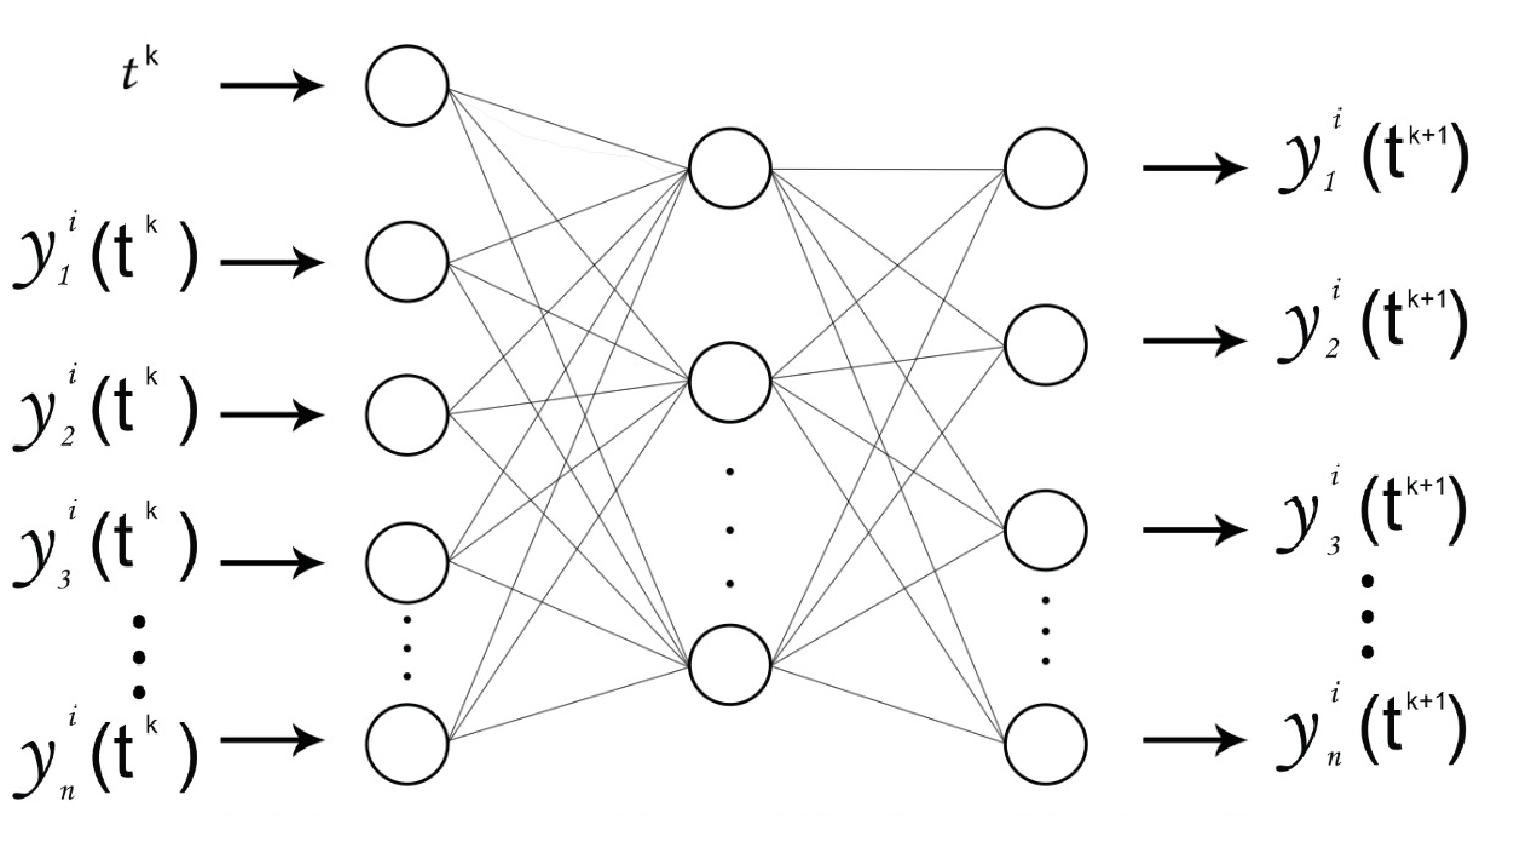
\includegraphics[scale=0.35]{Definitions/figure1.png}
	\caption{Basic scheme of the NARMAX methodology designed on a feed-forward neural architecture (Source: see \cite{ref5, ref6}).}	
	\label{fig1}
\end{figure}

\begin{figure}[htb]
	\centering
	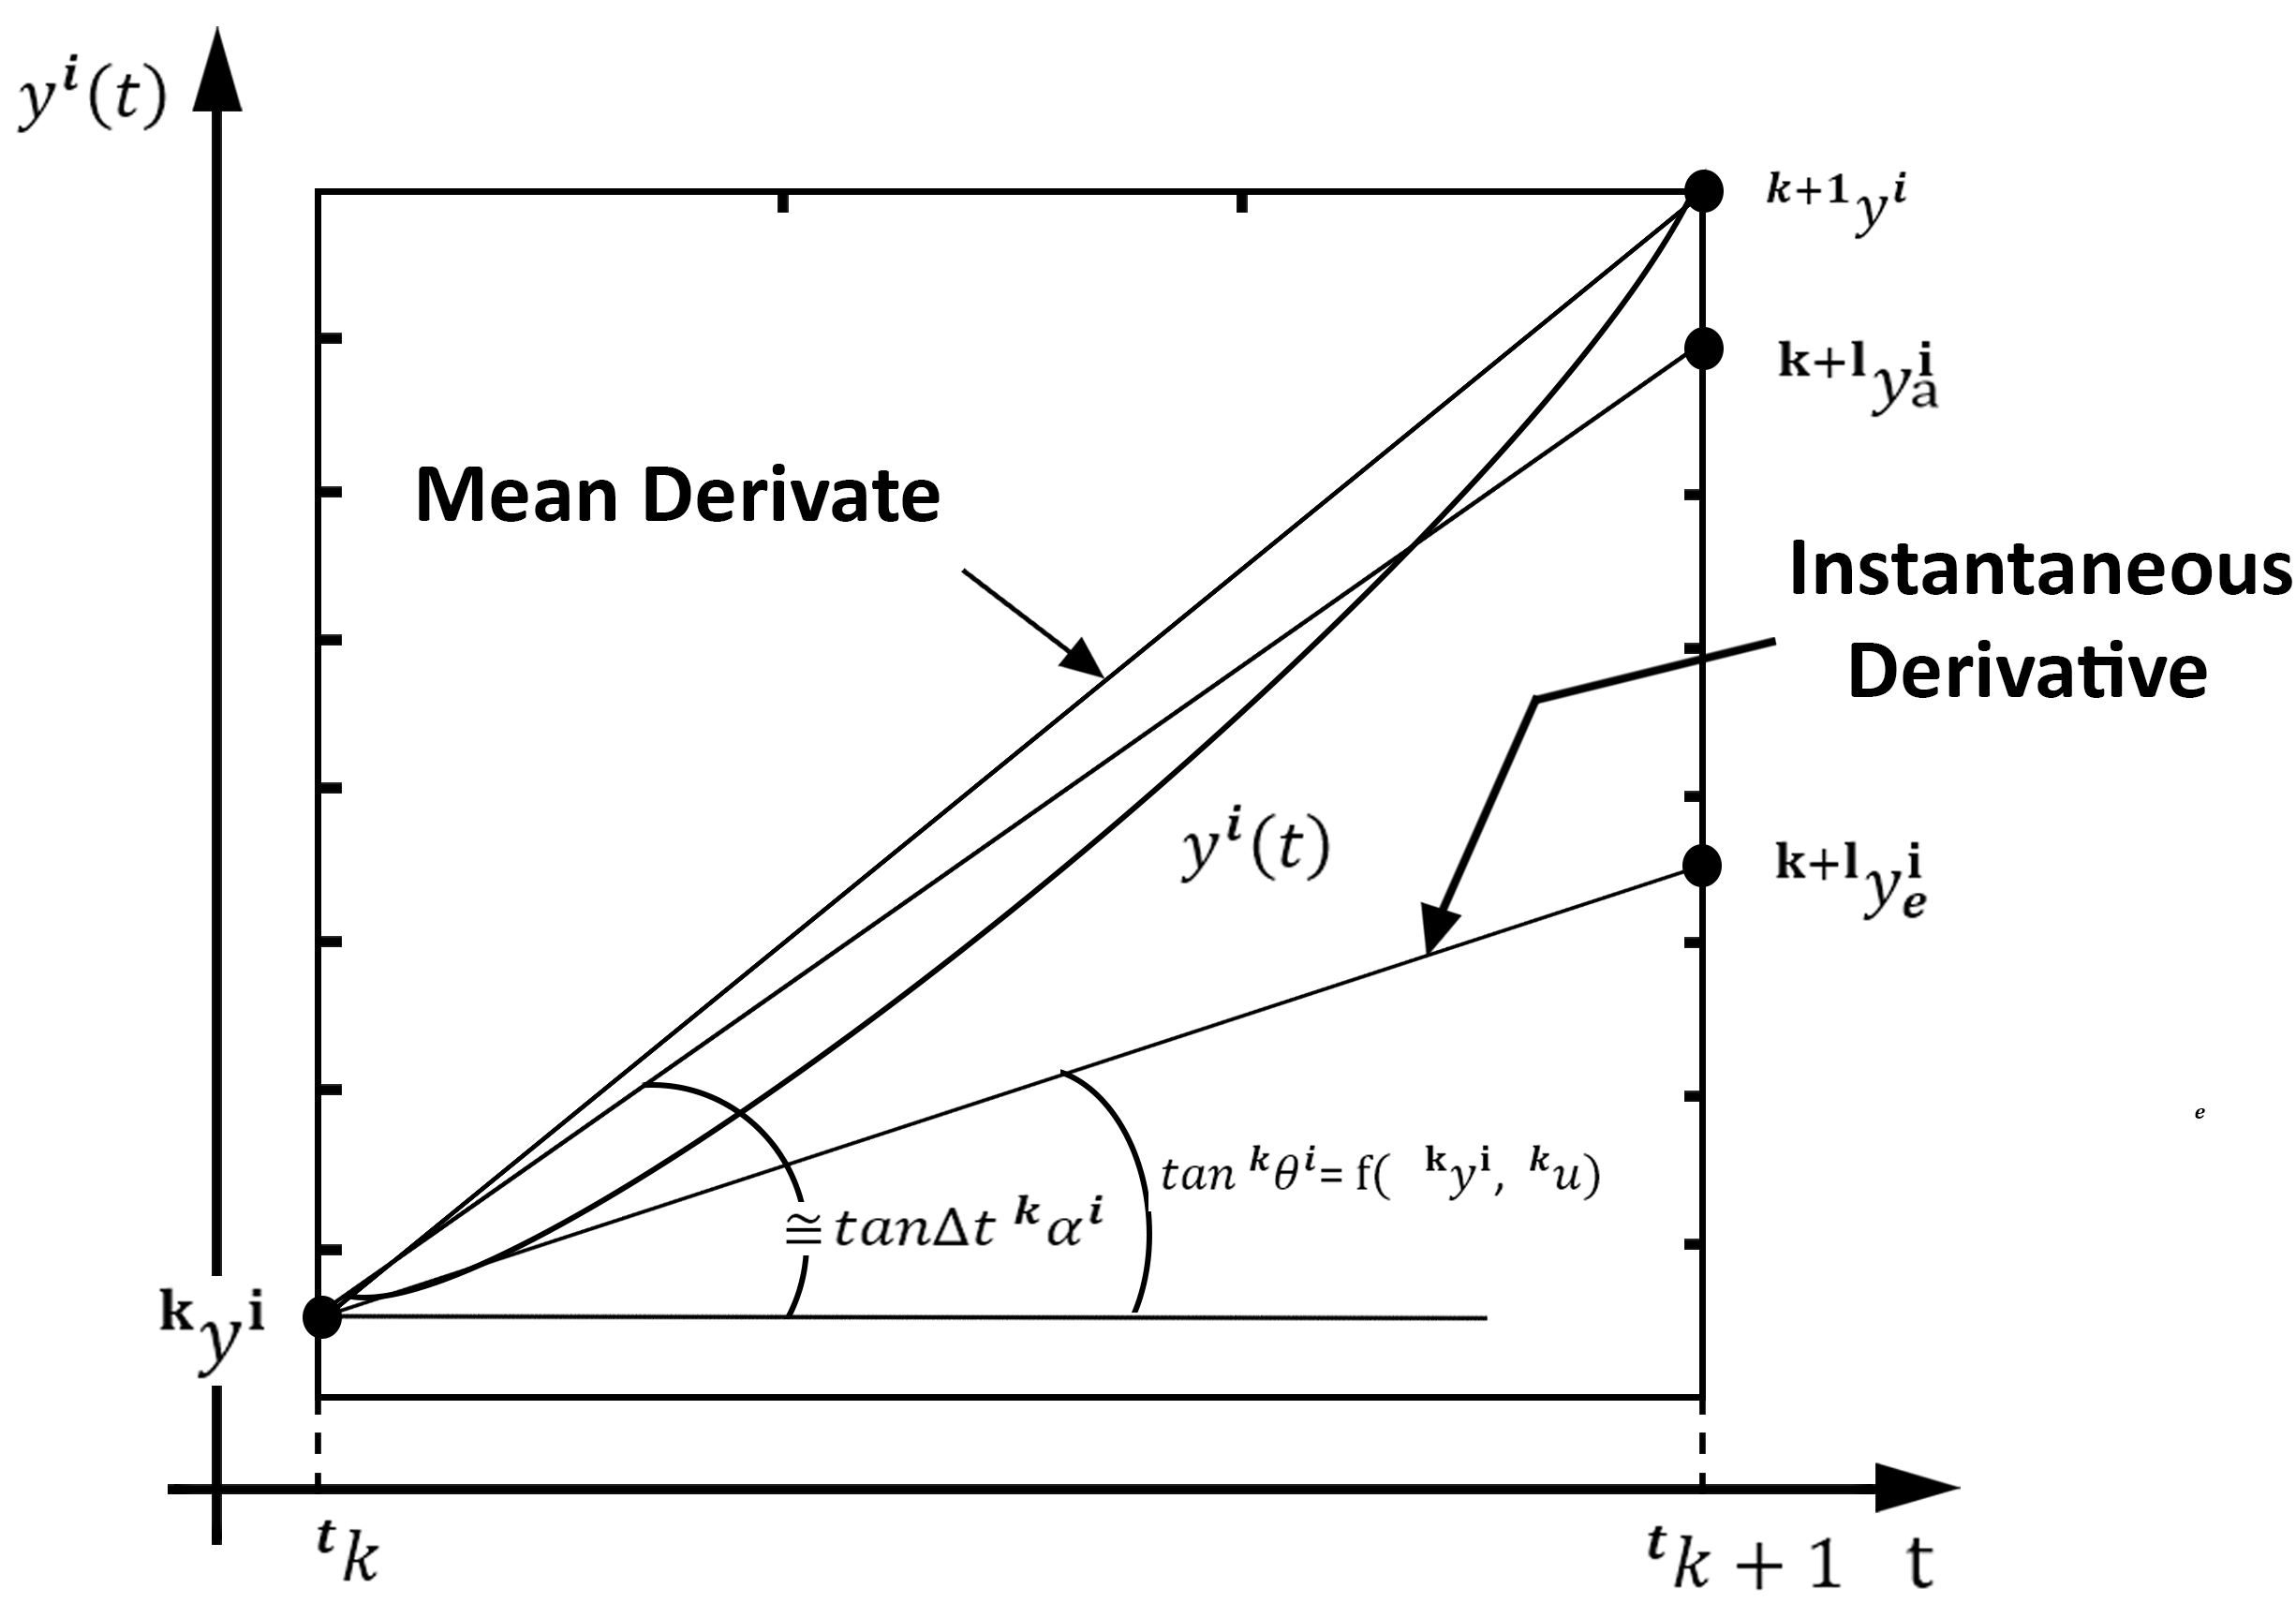
\includegraphics[scale=0.17]{Definitions/figure2.png}
	\caption{Difference between mean derivative and instantaneous derivative functions (Source: see \cite{ref7, ref8}).}
	\label{fig2}
\end{figure}

\begin{figure}[htb]
\centering
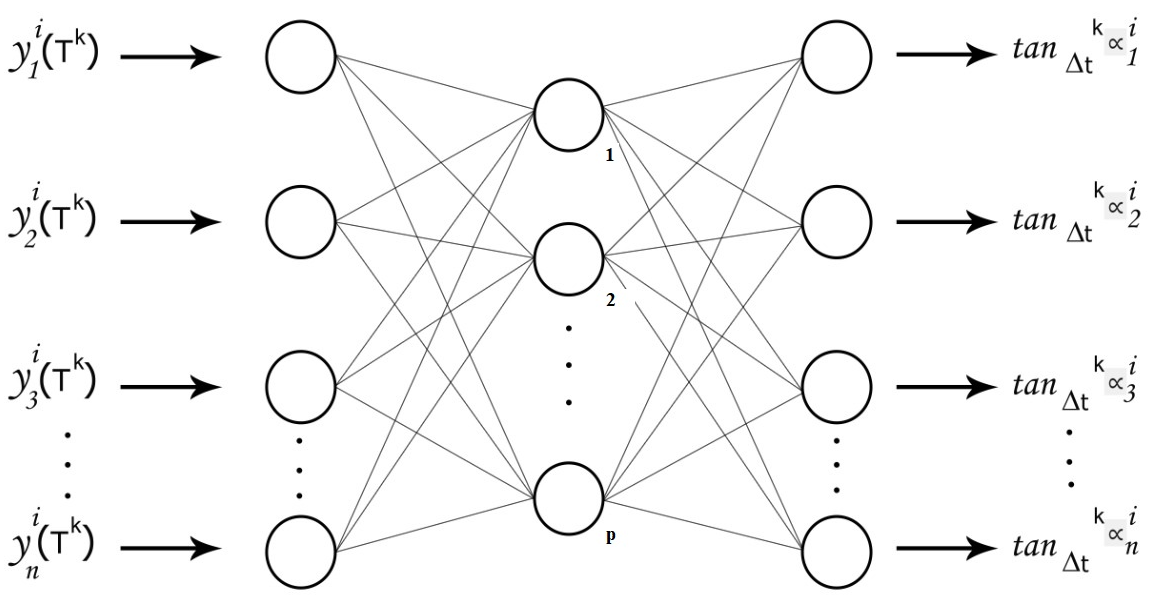
\includegraphics[scale=0.46]{Definitions/figure3.png}
\caption{A feed-forward neural network project with the concept of mean derivative functions.}
\label{fig3}
\end{figure}

\begin{figure}[htb]
\centering
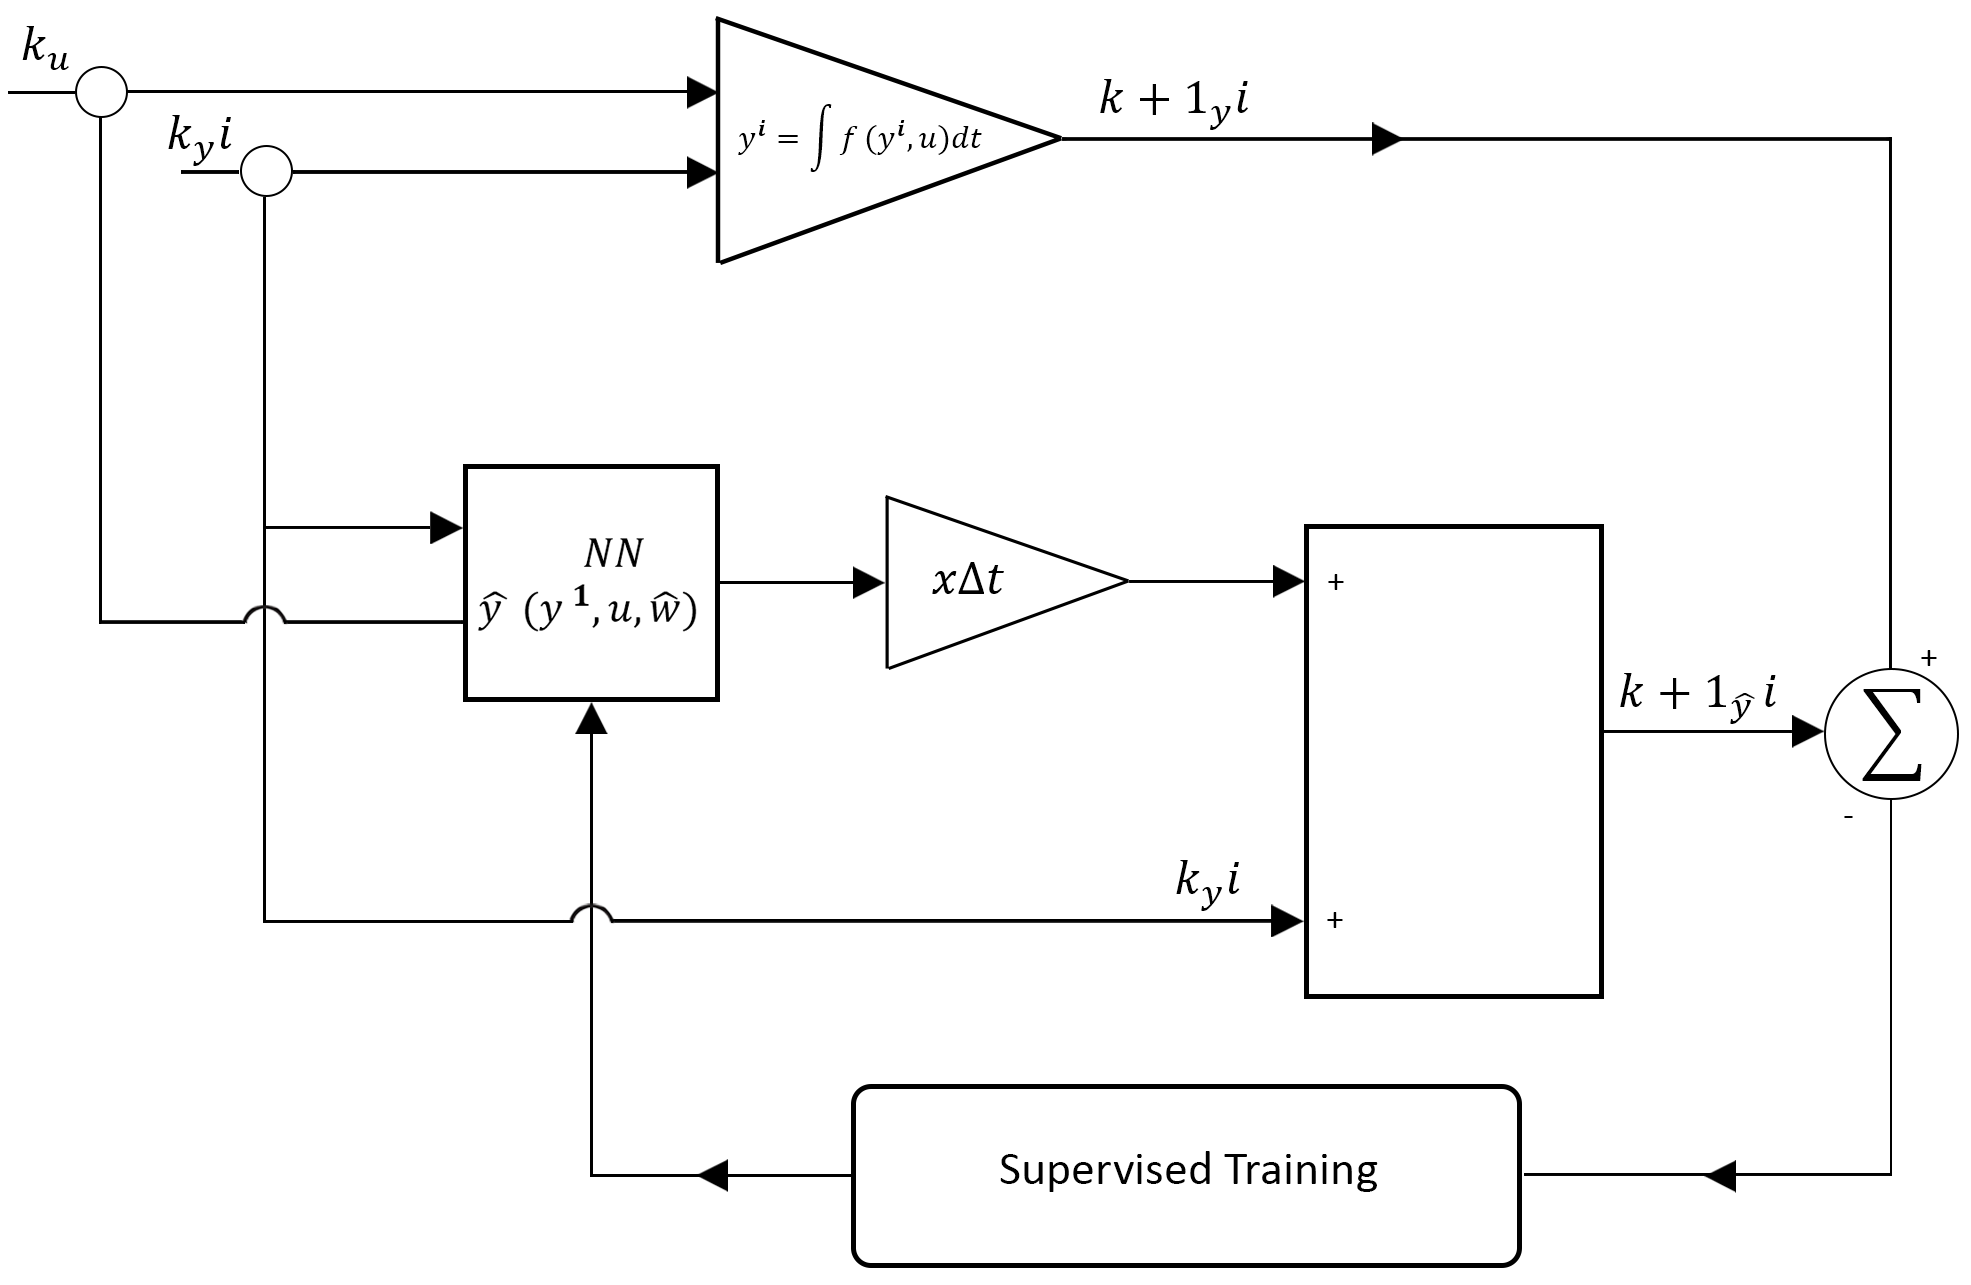
\includegraphics[scale=0.24]{Definitions/figure4.png}
\caption{Basic scheme of a feed-forward network designed internally in the Runge-Kutta 4-5 integrator (Source: see \cite{ref11}).}
\label{fig4}
\end{figure}

\begin{figure}[htb]
\centering
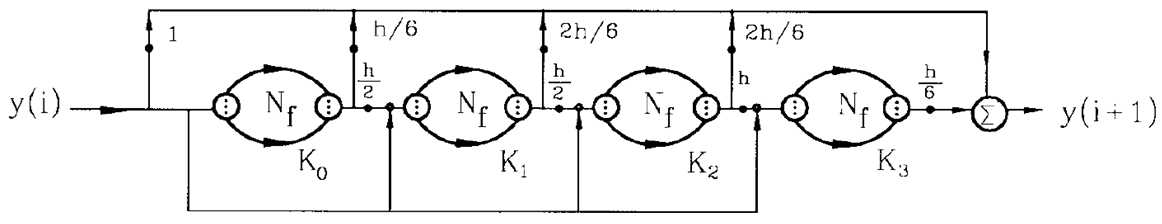
\includegraphics[scale=0.55]{Definitions/figure5.png}
\caption{Basic scheme of a feed-forward network designed internally in the Adams-Bashforth 4 integrator (Source: see \cite{ref12}).}
\label{fig5}
\end{figure}

\begin{equation}
	\left\{\begin{matrix}
		\dot{y}_1= f_1(t, y_1, y_2, \cdots y_n), & y_1(a)=\eta _1 \\
 		\dot{y}_2= f_2(t, y_1, y_2, \cdots y_n), & y_2(a)=\eta _2 \\
 		\vdots & \vdots \\
 		\dot{y}_n= f_n(t, y_1, y_2, \cdots y_n), & y_n(a)=\eta _n 
	\end{matrix}\right.	
	\label{eq:1}
 \end{equation}

Thus, a NARMAX model (no input with noise) of the Single-Input and Single-Output (SISO) type is given by \cite{ref5, ref6}:

$$ \hat{y}(k+1)=H[\varphi (k)]= $$
\begin{equation}
	\hat{f}_{NN}
	\begin{bmatrix} y(k) & \cdots & y(k-n_y) & u(k) & \cdots & u(k-n_u)
	\end{bmatrix}
	\label{eq:2}
\end{equation}

Furthermore, the NARMAX model can also be easily extended to the Multiple-Input and Multiple-Output (MIMO) case. For example, if $ \vec{y}(k-i)= $ $ [y_1(k-i) $ $ y_2(k-i) $ $ \cdots $ $ y_n(k-i)]^T $ e $ \vec{u}(k-j )= $ $ [u_1(k-j) $ $ u_2(k-j) $ $ \cdots $ $ u_n(k-j)]^T $ then one would have the following:

\begin{center}
	$ [\hat{\vec{y}}(k+1) $ $ \hat{\vec{y}}(k+2) $ $ \cdots $ $ \hat{\vec{y}}(k+n_{y_{out }})]= $
\end{center}
\begin{equation}
	\hat{f}_{NN}[\quad \vec{y}(k) \quad \vec{y}(k-1) \quad \cdots \quad \vec{y}(k-n_{y_{in}}) \quad  
	\begin{matrix}
		\vec{u}(k) & \vec{u}(k-1) & \cdots & \vec{u}(k-n_{u})
	\end{matrix}]^T
	\label{eq:3}
\end{equation}

There is also the mean derivatives methodology, which is an alternative to the NARMAX model \cite{ref7, ref8, ref9}. This type of integrator couples a feed-forward neural network to the first-order Euler integrator and as schematized by equations (\ref{eq:4}) and (\ref{eq:5}).

\begin{equation}
{^{k + 1}y^i} = tan_{\Delta t} {^{k}\alpha^i} \cdot \Delta t + {^{k}y^i}
\label{eq:4}
\end{equation}

\noindent where $ {^{k + 1}y^i}= $ $ [ $ $ {^{k + 1}y_1^i} $ $ {^{k + 2}y_2^i} $ $ \cdots $ $ {^{k + 1}y_n^i} $ $ ]^T $, $ tan_{\Delta t} {^{k + 1} \alpha^i}= $ $ [ $ $ tan_{\Delta t} {^{k + 1} \alpha_1^i} $ $ tan_{\Delta t} {^{k + 1} \alpha_2^i} $ $ \cdots $ $ tan_{\Delta t} {^{k + 1 } \alpha_n^i} $ $ ]^T$ and $ {^{k }y^i}= $ $ [ $ $ {^{k}y_1^i} $ $ {^{k}y_2^i} $ $ \cdots $ $ {^{k}y_n^i} $ $ ]^T $.

\begin{equation}
   tan_{\Delta t} {^{k}\alpha_j^i} = \frac{{^{k+1}y_j^i}-{^{k}y_j^i}}{\Delta t}
\label{eq:5}
\end{equation}

The only Runge-Kutta Neural Network (RKNN) that is available in the literature is the order 4-5 \cite{ref11}:

\begin{equation}
	y_{n+1}= y_n + \frac{h}{6}\cdot(k_1+ 2 \cdot k_2 + 2 \cdot k_3 + k_4)
	\label{eq:6}
\end{equation}

\noindent where,
$$ k_1= N_f(y_n;w) $$
$$ k_2= N_f(y_n + \frac{h}{2}\cdot k_1;w) $$
$$ k_3= N_f(y_n + \frac{h}{2}\cdot k_2;w) $$
$$ k_3= N_f(t_n + h, y_n +{h}\cdot k_3;w) $$
$$ N_f( \cdot, \cdot ;w) \cong \dot{y}=f(y(t))$$

Alternatively, there is also the Adams-Bashforth Neural Network (ABNN) which is also available in the literature and is given by \cite{ref12}:

\begin{equation}
	y(t_{n+1})=y(t_n)+ \frac{h}{24} \cdot (55 \cdot f_{n} - 59 \cdot f_{n-1} + 37 \cdot f_{n -2} - 9 \cdot f_{n-3})
	\label{eq:7}
\end{equation}

\subsection{Detailed Description of the Brazilian Financial Stock Market}

Section 3.2 goes here.


\subsection{Methodology Using Only One MLP Neural Network}

Section 3.3 goes here.



\subsection{The Proposed Method Using Multiple Neural Networks with MLP Architecture}

Section 3.4 goes here.



\section{Results and Analysis}

Here goes the Results and Experiments Section.

\subsection{Simple Method}

Section 4.1 goes here.

\subsection{Compound Method}

Section 4.2 goes here.

\subsection{Numerical and Computational Comparisons Between the Two Proposed Methodologies}

Section 4.3 goes here.

\section{Conclusion}

Here goes the Conclusion.


% Paulo Marcelo Tasinaffo está citando \cite{ref1, ref2, ref3, ref4, ref5, ref6, ref7, ref8, ref9, ref10, ref11, ref12, ref13, ref14, ref15, ref16, ref17, ref18, ref19, ref20, ref21, ref22, ref23, ref24, ref25, ref26, ref27, ref28, ref29, ref30, ref31, ref32, ref33, ref34, ref35, ref36, ref37, ref38, ref39, ref40}.

%%%%%%%%%%%%%%%%%%%%%%%%%%%%%%%%%%%%%%%%%%
\vspace{6pt} 

%%%%%%%%%%%%%%%%%%%%%%%%%%%%%%%%%%%%%%%%%%
%% optional
%\supplementary{The following supporting information can be downloaded at:  \linksupplementary{s1}, Figure S1: title; Table S1: title; Video S1: title.}

% Only for journal Methods and Protocols:
% If you wish to submit a video article, please do so with any other supplementary material.
% \supplementary{The following supporting information can be downloaded at: \linksupplementary{s1}, Figure S1: title; Table S1: title; Video S1: title. A supporting video article is available at doi: link.}

% Only for journal Hardware:
% If you wish to submit a video article, please do so with any other supplementary material.
% \supplementary{The following supporting information can be downloaded at: \linksupplementary{s1}, Figure S1: title; Table S1: title; Video S1: title.\vspace{6pt}\\
%\begin{tabularx}{\textwidth}{lll}
%\toprule
%\textbf{Name} & \textbf{Type} & \textbf{Description} \\
%\midrule
%S1 & Python script (.py) & Script of python source code used in XX \\
%S2 & Text (.txt) & Script of modelling code used to make Figure X \\
%S3 & Text (.txt) & Raw data from experiment X \\
%S4 & Video (.mp4) & Video demonstrating the hardware in use \\
%... & ... & ... \\
%\bottomrule
%\end{tabularx}
%}

%%%%%%%%%%%%%%%%%%%%%%%%%%%%%%%%%%%%%%%%%%

\authorcontributions{Methodology, software, and writing was made by P. T.; supervision and project administration, L. D. All authors have read and agree to the published version of the manuscript.}

\funding{The authors thank the Brazilian Aeronautics Institute of Technology (Instituto Tecnológico de Aeronáutica - ITA); the Casimiro Montenegro Filho Foundation (Fundação Casimiro Montenegro Filho - FCMF); and the Brazilian Enterprise Ecossistema Negócios Digitais Ltda for their support and infrastructure, which motivate the challenges and innovations of this research project.}

\institutionalreview{Not applicable.}

\informedconsent{Not applicable.}

\dataavailability{Not applicable.} 

% Only for journal Nursing Reports
%\publicinvolvement{Please describe how the public (patients, consumers, carers) were involved in the research. Consider reporting against the GRIPP2 (Guidance for Reporting Involvement of Patients and the Public) checklist. If the public were not involved in any aspect of the research add: ``No public involvement in any aspect of this research''.}

% Only for journal Nursing Reports
%\guidelinesstandards{Please add a statement indicating which reporting guideline was used when drafting the report. For example, ``This manuscript was drafted against the XXX (the full name of reporting guidelines and citation) for XXX (type of research) research''. A complete list of reporting guidelines can be accessed via the equator network: \url{https://www.equator-network.org/}.}

\acknowledgments{I would like to thank Professors and great friends Atair Rios Neto and Adilson Marques da Cunha for their valuable tips for improving this article. Finally, I would also like to thank the valuable improvement tips given by the good reviewers of this journal. The authors of this article would also like to thank God for making all of this possible.}

\conflictsofinterest{The authors declare no conflict of interest.} 

%%%%%%%%%%%%%%%%%%%%%%%%%%%%%%%%%%%%%%%%%%
%% Optional
% \sampleavailability{Samples of the compounds ... are available from the authors.}

%% Only for journal Encyclopedia
%\entrylink{The Link to this entry published on the encyclopedia platform.}

\abbreviations{Abbreviations}{
The following abbreviations are used in this manuscript:\\

\noindent 
\begin{tabular}{@{}ll}
ABNN     &  Adams-Bashforth Neural Network\\
E-TUNI   &  Euler-Type Universal Numerical Integrator\\
NARMAX   &  Nonlinear Auto Regressive Moving Average with eXogenous input\\
MLP      &  Multi-Layer Perceptron\\
PCNN     &  Predictive-Corrector Neural Network\\
RBF      &  Radial Basis Function\\
RKNN     &  Runge-Kutta Neural Network\\
SVM      &  Support Vector Machine\\  
UNI      &  Universal Numerical Integrator
\end{tabular}
}

%%%%%%%%%%%%%%%%%%%%%%%%%%%%%%%%%%%%%%%%%%
\begin{adjustwidth}{-\extralength}{0cm}
%\printendnotes[custom] % Un-comment to print a list of endnotes

\reftitle{References}

% Please provide either the correct journal abbreviation (e.g. according to the “List of Title Word Abbreviations” http://www.issn.org/services/online-services/access-to-the-ltwa/) or the full name of the journal.
% Citations and References in Supplementary files are permitted provided that they also appear in the reference list here. 

%=====================================
% References, variant A: external bibliography
%=====================================
%\bibliography{your_external_BibTeX_file}

%=====================================
% References, variant B: internal bibliography
%=====================================
\begin{thebibliography}{999}

% Reference 1
\bibitem[Author1(year)]{ref1}
Cybenko, G. \textit{Continuous Valued Networks with Two Hidden Layers Are Sufficient}. University of Illinois at Urbana-Champaign: Center for Supercomputing Research and Development, 1988.

% Reference 2
\bibitem[Author2(year)]{ref2}
Hornik, K.; Stinchcombe, M.; White, H. Multilayer feedforward networks are universal approximators. {\em Neural Networks} {\bf 1989}, {\em 2(5)}, 359--366.

% Reference 3
\bibitem[Author3(year)]{ref3}
Haykin, S. \textit{Neural Networks: A Comprehensive Foundation}. Publisher: Prentice-Hall, Inc., New Jersey, USA, 1999.

% Reference 4
\bibitem[Author4(year)]{ref4}
Tasinaffo, P. M.; Gonçalves, G. S.; Cunha, A. M.; Dias, L. A. V. An introduction to universal numerical integrators. {\em Int. J. Innov. Comput. Inf. Control} {\bf 2019}, {\em 15(1)}, 383--406.

% Reference 5
\bibitem[Author5(year)]{ref5}
Billings, S. A.; Chen, S.; Koreberg, M. J. Identification of {MIMO} non-linear systems using forward-regression orthogonal estimator. {\em Int. J. Control} {\bf 1989}, {\em 49(6)}, 2157--2189.

% Reference 6
\bibitem[Author6(year)]{ref6}
Chen, S. and Billings; S. A. Neural networks for nonlinear dynamic system modelling and identification. {\em Int. J. Control} {\bf 1992}, {\em 56(2)}, 319--346.

% Reference 7
\bibitem[Author7(year)]{ref7}
Tasinaffo, P. M. Estruturas de Integração Neural Feedforward Testadas em Problemas de Controle Preditivo. Doctoral Thesis, INPE-10475-TDI/945, São José dos Campos/SP, Brazil, 2003.

% Reference 8
\bibitem[Author8(year)]{ref8}
Tasinaffo, P. M.; Rios Neto, A. Mean derivatives based neural {E}uler integrator for nonlinear dynamic systems modeling. {\em Learning and Nonlinear Models} {\bf 2005}, {\em 3(2)}, 98--109.

% Reference 9
\bibitem[Author9(year)]{ref9}
de Figueiredo, M. O.; Tasinaffo, P. M.; Dias, L. A. V. Modeling autonomous nonlinear dynamic systems using mean derivatives, fuzzy logic and genetic algorithms. {\em Int. J. Innov. Comput. Inf. Control} {\bf 2016}, {\em 12(5)}, 1721--1743.


% Reference 10
\bibitem[Author10(year)]{ref10}
Vidyasagar, M. \textit{Nonlinear Systems Analysis}. Publisher: Prentice-Hall, Inc., Electrical Engineering Series, New Jersey, USA, 1978.

% Reference 11
\bibitem[Author11(year)]{ref11}
Wang, Y.-J.; Lin, C.-T. Runge-{K}utta neural network for identification of dynamical systems in high accuracy. {\em IEEE Transactions on Neural Networks} {\bf 1998}, {\em 9(2)}, 294--307.

% Reference 12
\bibitem[Author12(year)]{ref12}
Tasinaffo, P. M.; Rios Neto, A. Adams-{B}ashforth neural networks applied in a predictive control structure with only one horizon. {\em Int. J. Innov. Comput. Inf. Control} {\bf 2019}, {\em 15(2)}, 445--464.

% Reference 13
\bibitem[Author13(year)]{ref13}
Chen, R. T. Q.; Rubanova, Y.; Bettencourt, J.; Duveand, D. Neural ordinary differential equations. In Proceedings of the 32nd Conference on Neural Information Processing Systems (NeurlPS), Montréal, Canada, 2018, 1--19.

% Reference 14
\bibitem[Author14(year)]{ref14}
Uçak, K. A {R}unge-{K}utta {MLP} neural network based control method for nonlinear {MIMO} systems. In Proceedings of the 6th International Conference on Electrical and Electronics Engineering (ICEEE), Istanbul, Turkey, 2019, 186-192.

% Reference 15
\bibitem[Author15(year)]{ref15}
Spooner, J. T.; Maggiore, M.; Ordónez, R.; Passino, K. M. \textit{Stable Adaptive Control and Estimation for Nonlinear Systems Neural and Fuzzy Approximator Techniques}. Publisher: Wiley-Interscience, New York, USA, 2002.

% Reference 16
\bibitem[Author16(year)]{ref16}
Hagan, M. T.; Menhaj, M. B Training feedforward networks with the Marquardt algorithm. {\em IEEE Transactions on Neural Networks} {\bf 1994}, {\em 5(6)}, 989--993.


% Reference 6
%\bibitem[Author6(year)]{ref6}
%Hornik, K.; Stinchcombe, M.; White, H. Multilayer feedforward networks are universal approximators. {\em Neural Networks} {\bf 1989}, {\em 2(5)}, 359--366.

% Reference 7
%\bibitem[Author7(year)]{ref7}
%Haykin, S. \textit{Neural Networks: A Comprehensive Foundation}. Publisher: Prentice-Hall, Inc., New Jersey, USA, 1999.

% Reference 8
%\bibitem[Author8(year)]{ref8}
%Author 1, A.B.; Author 2, C.D.; Author 3, E.F. Title of presentation. In Proceedings of the Name of the Conference, Location of Conference, Country, Date of Conference (Day Month Year); Abstract Number (optional), Pagination (optional).

% Reference 9
%\bibitem[Author9(year)]{ref9}
%Author 1, A.B. Title of Thesis. Level of Thesis, Degree-Granting University, Location of University, Date of Completion.

\end{thebibliography}

% If authors have biography, please use the format below
%\section*{Short Biography of Authors}
%\bio
%{\raisebox{-0.35cm}{\includegraphics[width=3.5cm,height=5.3cm,clip,keepaspectratio]{Definitions/author1.pdf}}}
%{\textbf{Firstname Lastname} Biography of first author}
%
%\bio
%{\raisebox{-0.35cm}{\includegraphics[width=3.5cm,height=5.3cm,clip,keepaspectratio]{Definitions/author2.jpg}}}
%{\textbf{Firstname Lastname} Biography of second author}

% For the MDPI journals use author-date citation, please follow the formatting guidelines on http://www.mdpi.com/authors/references
% To cite two works by the same author: \citeauthor{ref-journal-1a} (\citeyear{ref-journal-1a}, \citeyear{ref-journal-1b}). This produces: Whittaker (1967, 1975)
% To cite two works by the same author with specific pages: \citeauthor{ref-journal-3a} (\citeyear{ref-journal-3a}, p. 328; \citeyear{ref-journal-3b}, p.475). This produces: Wong (1999, p. 328; 2000, p. 475)

%%%%%%%%%%%%%%%%%%%%%%%%%%%%%%%%%%%%%%%%%%
%% for journal Sci
%\reviewreports{\\
%Reviewer 1 comments and authors’ response\\
%Reviewer 2 comments and authors’ response\\
%Reviewer 3 comments and authors’ response
%}
%%%%%%%%%%%%%%%%%%%%%%%%%%%%%%%%%%%%%%%%%%
\PublishersNote{}
\end{adjustwidth}
\end{document}

